% ПРОЧИТАЙ МЕНЯ
% ПРОЧИТАЙ МЕНЯ
% ПРОЧИТАЙ МЕНЯ
%
% В этом файле вы описываете задачи из контеста
% Условия можно вставить в виде фотографий
% В идеях нужно написать хотя бы два-три предложения о задаче
% Если задача довольно трудная, описание идеи должно быть подробным
% Комментарии в исходном коде приветствуются
% Положение тоже можно фотографией
%
% ПРОЧИТАЙ МЕНЯ
% ПРОЧИТАЙ МЕНЯ
% ПРОЧИТАЙ МЕНЯ

\section{Отчёт обучающегося по практике}

\subsection*{Основы C++ [1] (Тренировочное соревнование)}
\begin{center} 
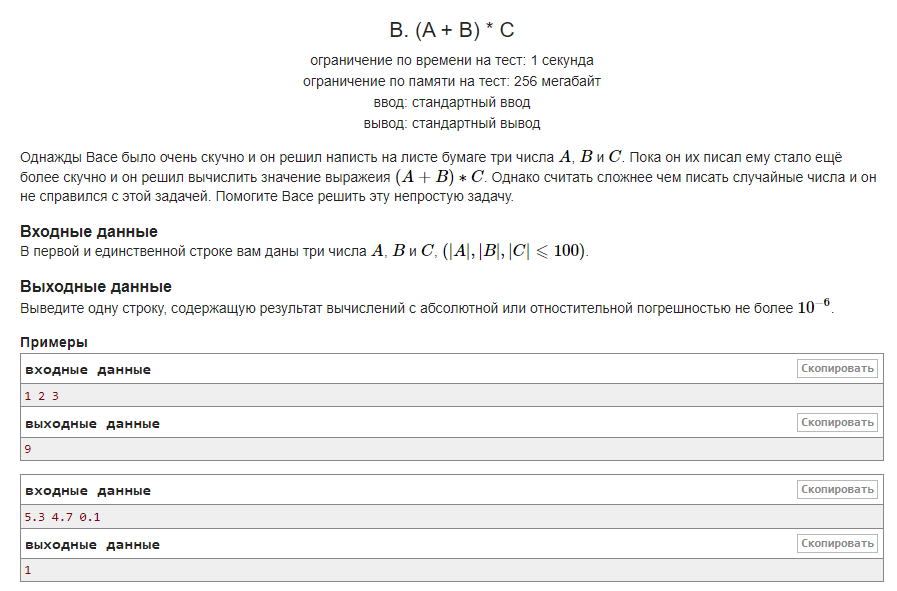
\includegraphics[scale=0.75]{statements/1_B.png}
\end{center} 
\subsubsection*{Идея}
Здесь мы вводим координаты двух противоположных улов обоих прямоугольников. Для упрощения значения нечетных переменных будут больше. Далее мы сравниваем координаты углов, чтобы правильно определить длину сторон их пересечения. И напоследок мы вычисляем площадь этого пересечения.

\subsubsection*{Исходный код}
\lstinputlisting{src/1TaskB.cpp}

\begin{center} 
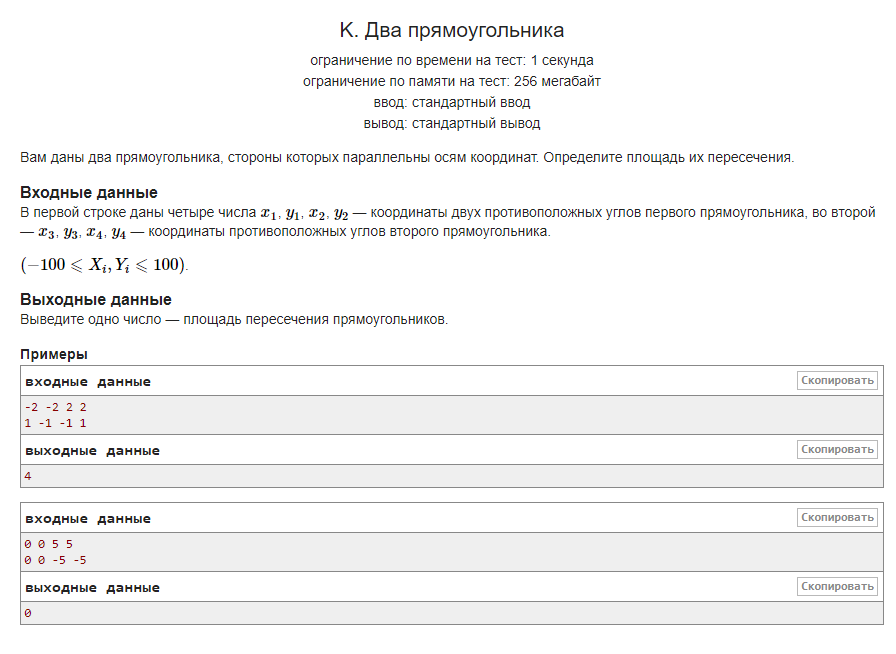
\includegraphics[scale=0.75]{summer-practice/statements/1_K.png}
\end{center} 
\subsubsection*{Идея}
Данная задача проще пареной репы. Сначала мы вводим переменные a, b и c, Затем мы выводим произведение суммы (a, b) и c.

\subsubsection*{Исходный код}
\lstinputlisting{src/1TaskK.cpp}


\subsubsection*{Фрагмент турнирной таблицы контеста}
\begin{center} 
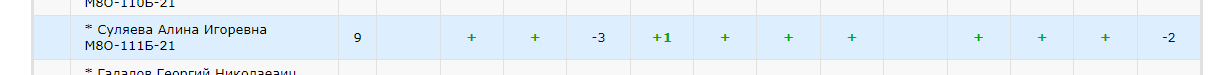
\includegraphics[scale=0.5]{standings/1.png}\newline\noindent
\end{center} 
\pagebreak

\subsection*{Основы C++ [2] (Тренировочное соревнование)}
\begin{center} 
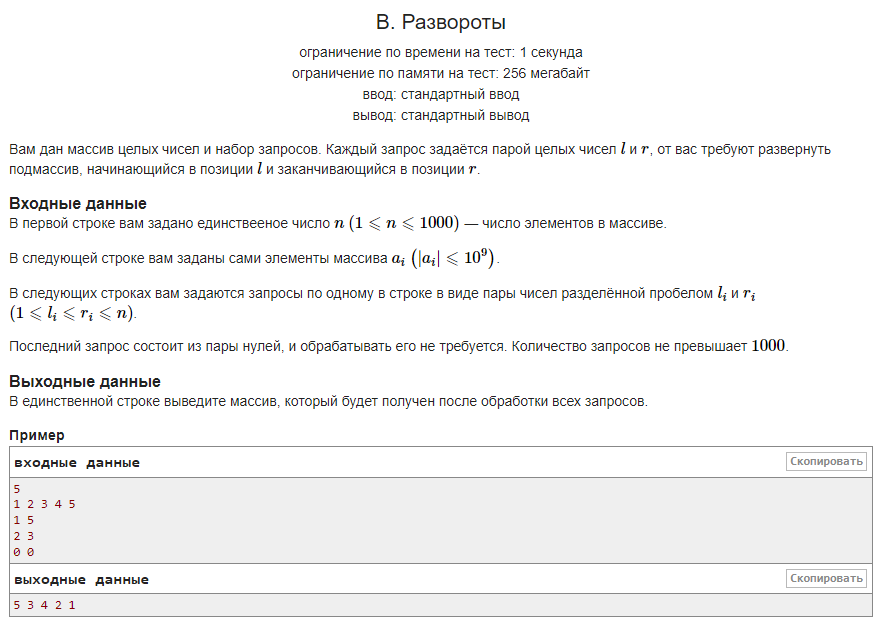
\includegraphics[scale=0.75]{statements/2_B.png}
\end{center} 
\subsubsection*{Идея}
В первую очередь мы вводим количество элементов в массиве, затем -- последовательность в массив, а затем записываем порядки элементов, которые мы поменяем местами. Далее мы производим операцию $swap$ нужных элементов (не забывая уменьшать индекс на 1). Далее мы выводим отсортированную последовательность.
\subsubsection*{Исходный код}
\lstinputlisting{src/2TaskB.cpp}


\subsubsection*{Фрагмент турнирной таблицы контеста}
\begin{center} 
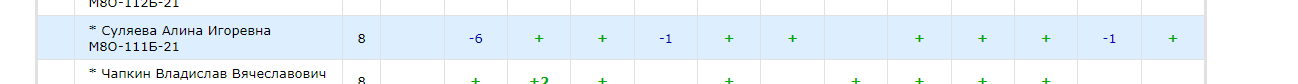
\includegraphics[scale=0.5]{standings/2.png}\newline\noindent
\end{center} 
\pagebreak

\subsection*{Библиотека C++ [1] (Тренировочное соревнование)}
\begin{center} 
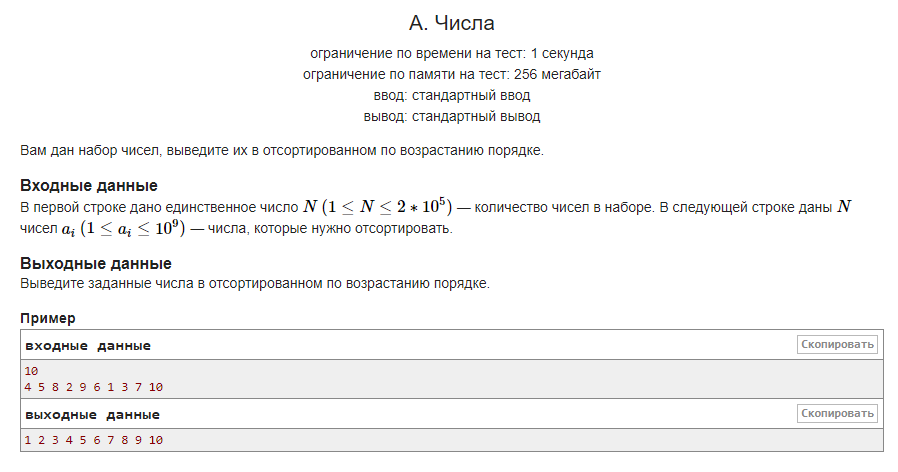
\includegraphics[scale=0.75]{statements/3_A.png}
\end{center} 
\subsubsection*{Идея}
В первую очередь мы вводим последовательность в вектор, а затем мы сортируем методом std::sort, он работает в среднем за $n \cdot log(n)$. Далее мы выводим отсортированную последовательность.
\subsubsection*{Исходный код}
\lstinputlisting{src/3TaskA.cpp}


\subsubsection*{Фрагмент турнирной таблицы контеста}
\begin{center} 
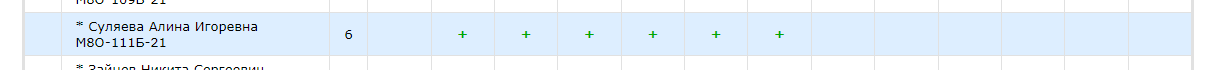
\includegraphics[scale=0.5]{standings/3.png}\newline\noindent
\end{center} 
\pagebreak

\subsection*{Библиотека C++ [2] (Тренировочное соревнование)}
\begin{center} 
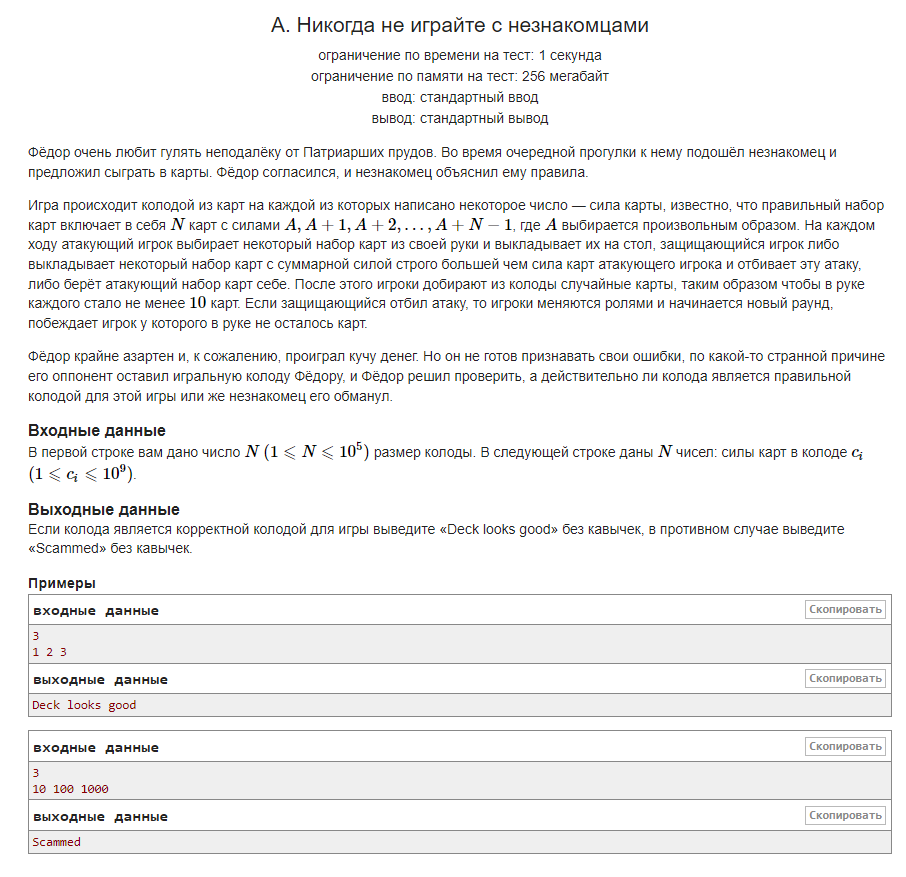
\includegraphics[scale=0.75]{statements/4_A.png}
\end{center} 
\subsubsection*{Идея}
В первую очередь мы вводим последовательность в вектор. Затем мы проверяем, заряжена ли колода в киосках: если в колоде одна карта или набор карт с значениями силы как в условии задачи (разница между соседними картами равна единице), то с колодой всё в порядке. В противном случае Федьку обманули...
\subsubsection*{Исходный код}
\lstinputlisting{src/4TaskA.cpp}


\subsubsection*{Фрагмент турнирной таблицы контеста}
\begin{center} 
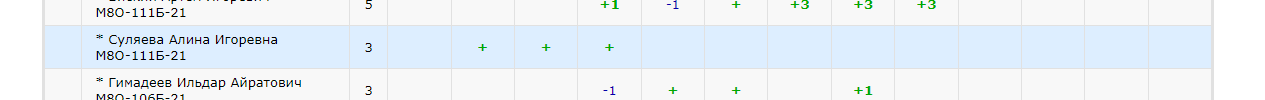
\includegraphics[scale=0.5]{standings/4.png}\newline\noindent
\end{center} 
\pagebreak

\subsection*{Теория чисел (Тренировочное соревнование)}
\begin{center} 
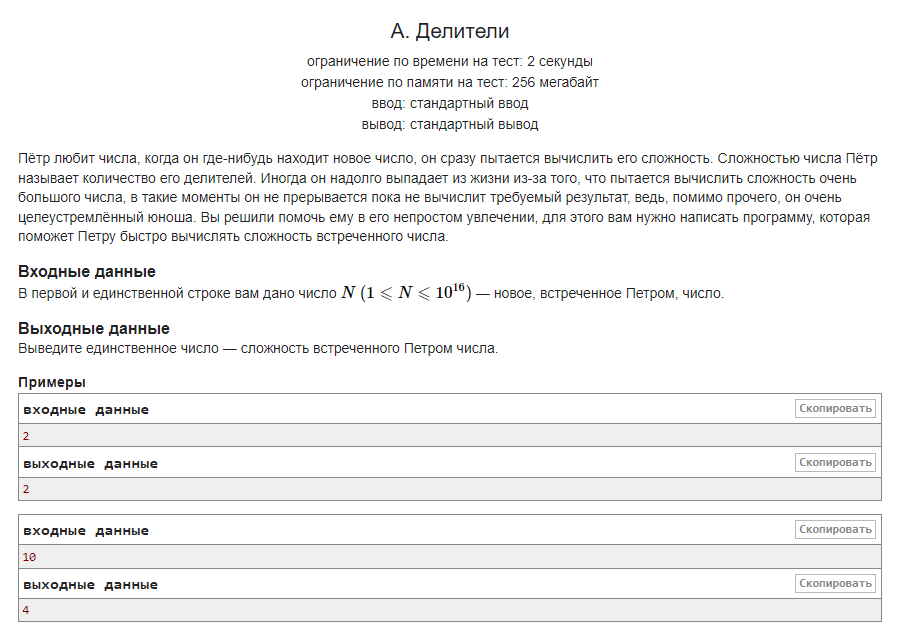
\includegraphics[scale=0.75]{statements/5_A.png}
\end{center} 
\subsubsection*{Идея}
Сначала мы вводим число, затем мы в цикле начинаем его делить, начиная с делителя 2. Если деление у нас без остатка, то к переменной ($tmp = 0$) мы прибавляем по единице за каждое деление нацело. Далее мы добавляем ещё одну единицу и умножаем переменную ответа ($res = 1$) на полученный результат $tmp$. Если делимое не является единицей, умножаем $res$ ещё на два и цикл продолжается до тех пор, пока условие не будет достигнуто. Во время этого делитель увеличивается на 1.
\subsubsection*{Исходный код}
\lstinputlisting{src/5TaskA.cpp}


\subsubsection*{Фрагмент турнирной таблицы контеста}
\begin{center} 
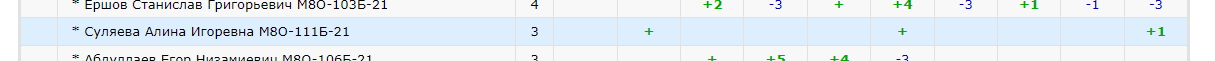
\includegraphics[scale=0.5]{standings/5.png}\newline\noindent
\end{center}
\pagebreak


\subsection*{Основы ДП (Тренировочное соревнование)}
\begin{center} 
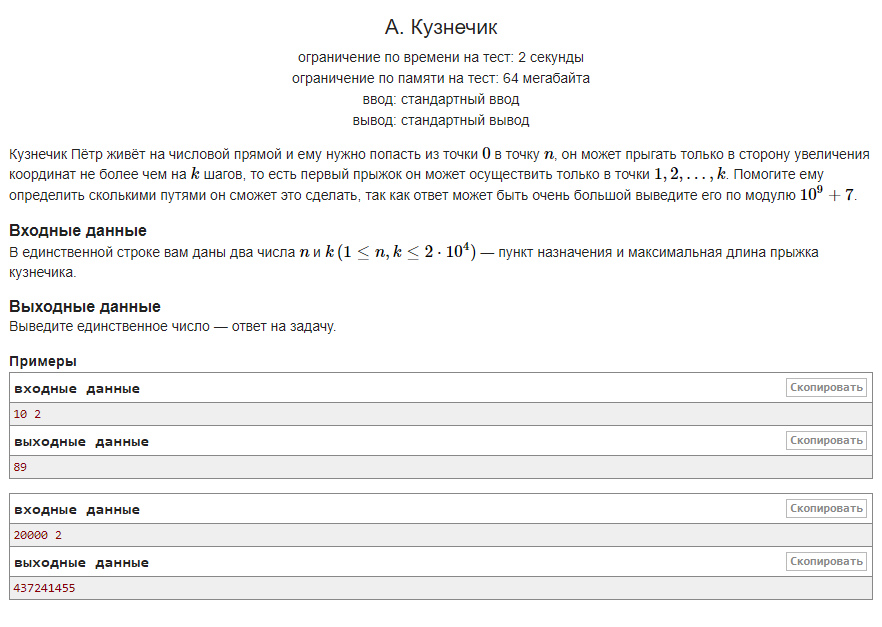
\includegraphics[scale=0.75]{statements/6_A.png}
\end{center} 
\subsubsection*{Идея}
Для решения этой задачи мы составляем таблицу результатов при движении на определённые координаты до значения $k$.
Значение ячейки в 0 и 1 координатах равны единице, дальнейшие ячейки вычисляется путём прибавления предыдущего шага в цикле ($i - j$), а затем берётся остаток от деления на $m$. Данные опперации позволяет не использовать рекурсию и упростить сложность. При завершении цикла выводим результат в предпоследней ячейке таблицы.
\subsubsection*{Исходный код}
\lstinputlisting{src/6TaskA.cpp}


\subsubsection*{Фрагмент турнирной таблицы контеста}
\begin{center} 
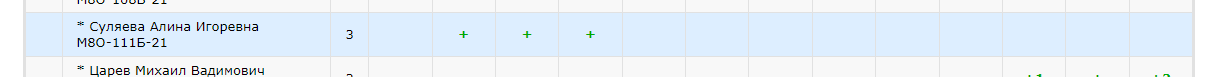
\includegraphics[scale=0.5]{standings/6.png}\newline\noindent
\end{center} 
\pagebreak

\subsection*{Арифметика в кольце, комбинаторика, функция Эйлера (Тренировочное соревнование)}
\begin{center} 
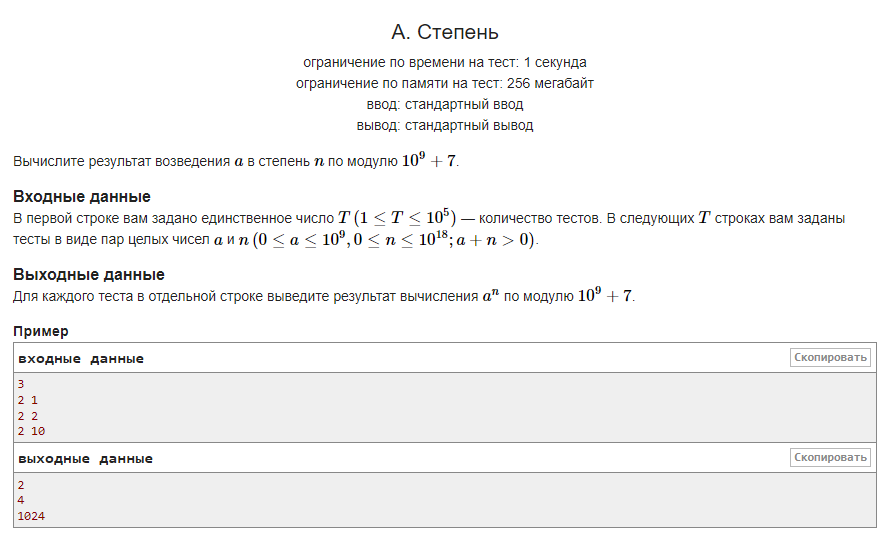
\includegraphics[scale=0.75]{statements/7_A.png}
\end{center} 
\subsubsection*{Идея}
Сначала мы вводим количество тестов, затем на каждый тест вводим число и степень, в которую мы возведём число. Далее мы производим бинарное возведение в степень, попутно не забывая про модуль.
\subsubsection*{Исходный код}
\lstinputlisting{src/7TaskA.cpp}


\subsubsection*{Фрагмент турнирной таблицы контеста}
\begin{center} 
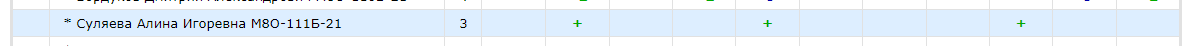
\includegraphics[scale=0.5]{standings/7.png}\newline\noindent
\end{center} 
\pagebreak

\subsection*{Префиксные суммы, сортировка событий, метод двух указателей (Тренировочное соревнование)}
\begin{center} 
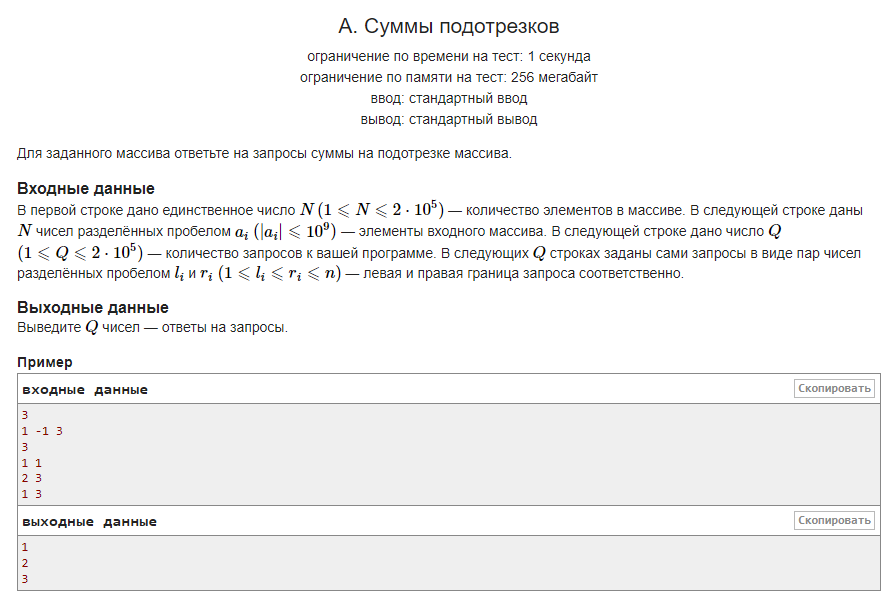
\includegraphics[scale=0.75]{statements/8_A.png}
\end{center} 
\subsubsection*{Идея}
Для решения этой задачи мы составляем таблицу результатов при движении на определённые координаты до значения $k$.
Значение ячейки в 0 и 1 координатах равны единице, дальнейшие ячейки вычисляется путём прибавления предыдущего шага в цикле ($i - j$), а затем берётся остаток от деления на $m$. Данные опперации позволяет не использовать рекурсию и упростить сложность. При завершении цикла выводим результат в предпоследней ячейке таблицы.
\subsubsection*{Исходный код}
\lstinputlisting{src/8TaskA.cpp}


\subsubsection*{Фрагмент турнирной таблицы контеста}
\begin{center} 
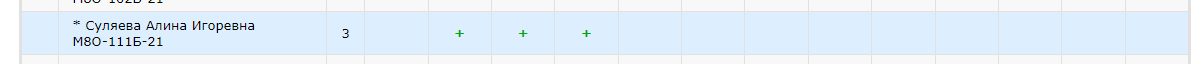
\includegraphics[scale=0.5]{standings/8.png}\newline\noindent
\end{center} 
\pagebreak

\section*{Grand Prix of Kyoto 20.02.2022}
В связи с недавними событиями данные недоступны
\subsection*{Идея}
В связи с недавними событиями данные недоступны
\subsection*{Исходный код}
В связи с недавними событиями данные недоступны
\subsection*{Фрагмент турнирной таблицы контеста}
В связи с недавними событиями данные недоступны
\newline\noindent
\pagebreak

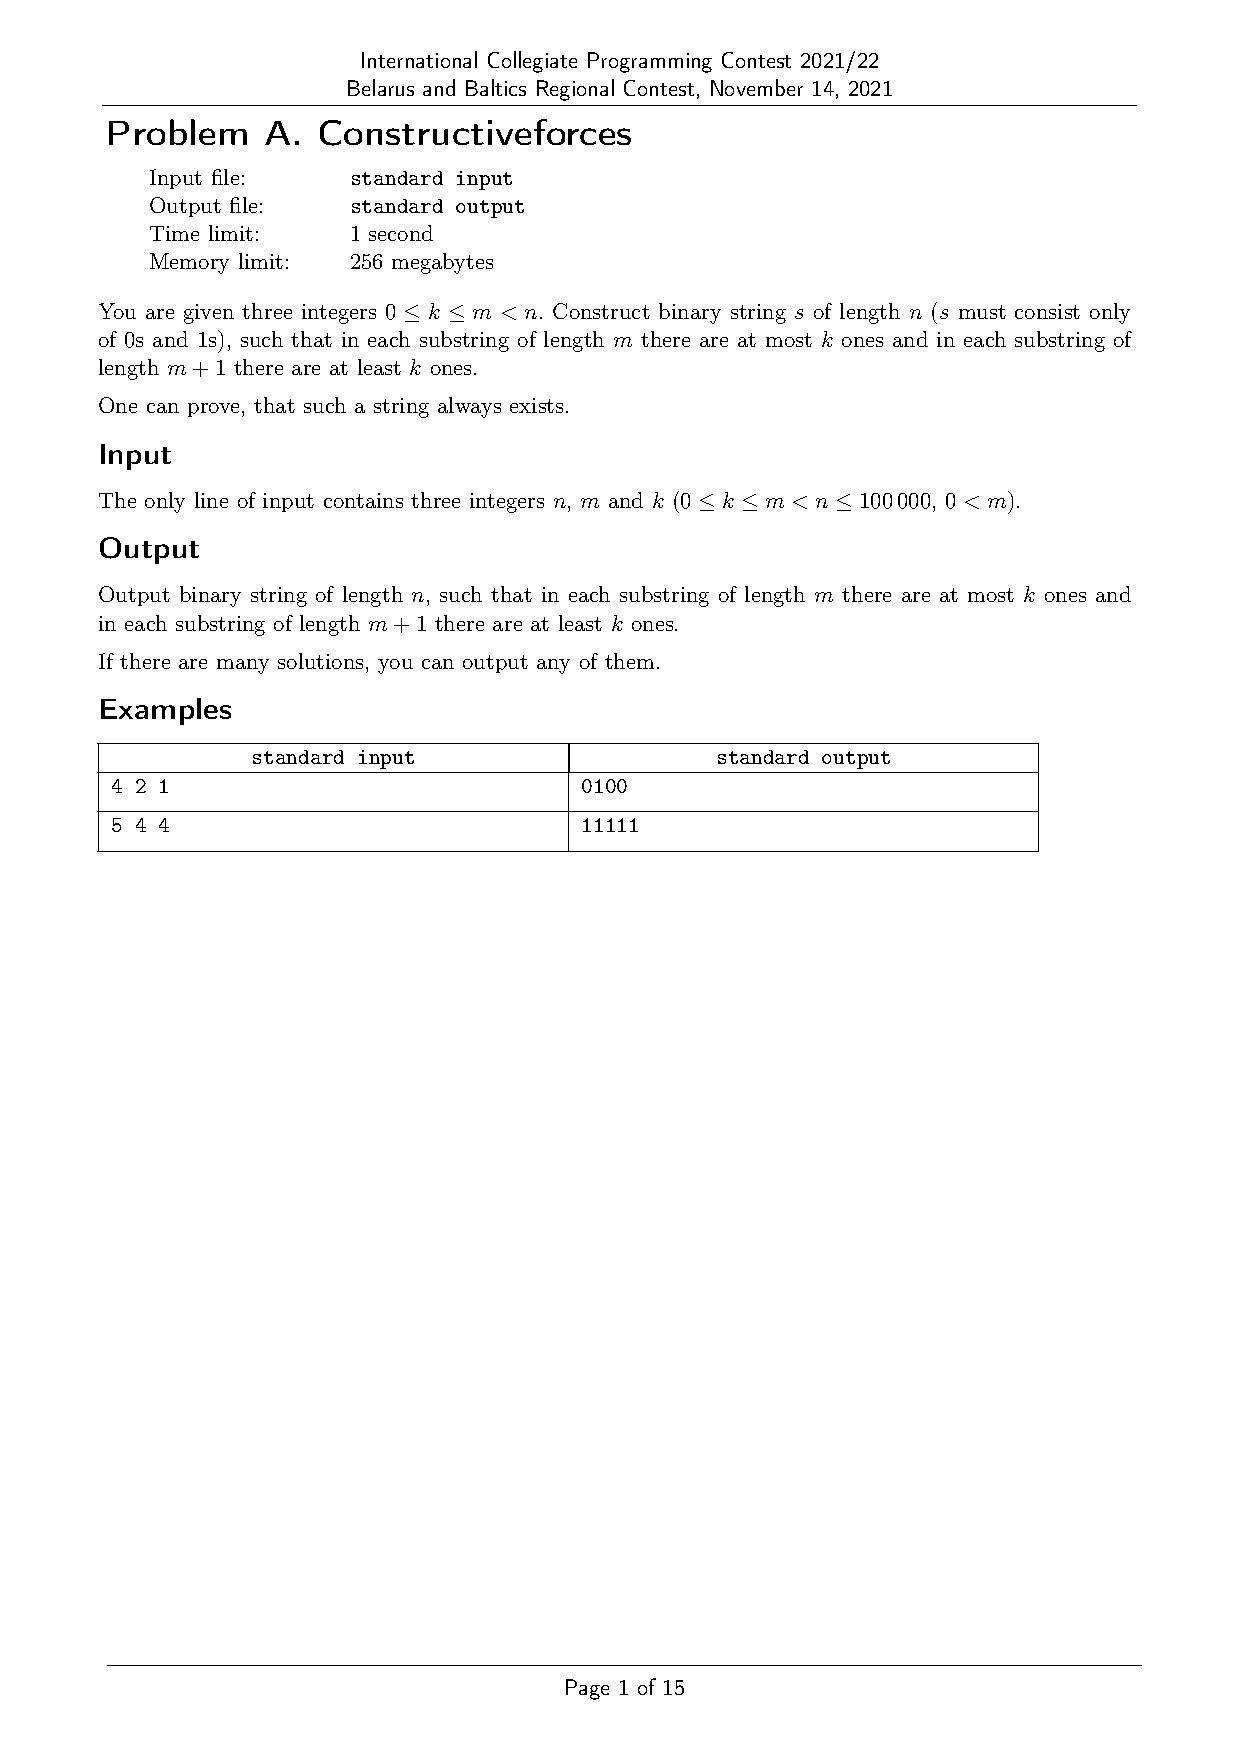
\includepdf[pages=1, scale=0.75, pagecommand=\section*{Regional 1. Belarus and Baltics 2021 13.03.2022 }]{statements/BBR2021.en.pdf}
\subsection*{Идея}
Сначала мы вводим элементы в массив, далее мы вычисляем сумму в данных подотрезках массива, не забывая про индекс - 1.
\subsection*{Исходный код}
\lstinputlisting[language=Python]{src/TaskA.py}
\subsection*{Фрагмент турнирной таблицы контеста}
Недоступно
\pagebreak

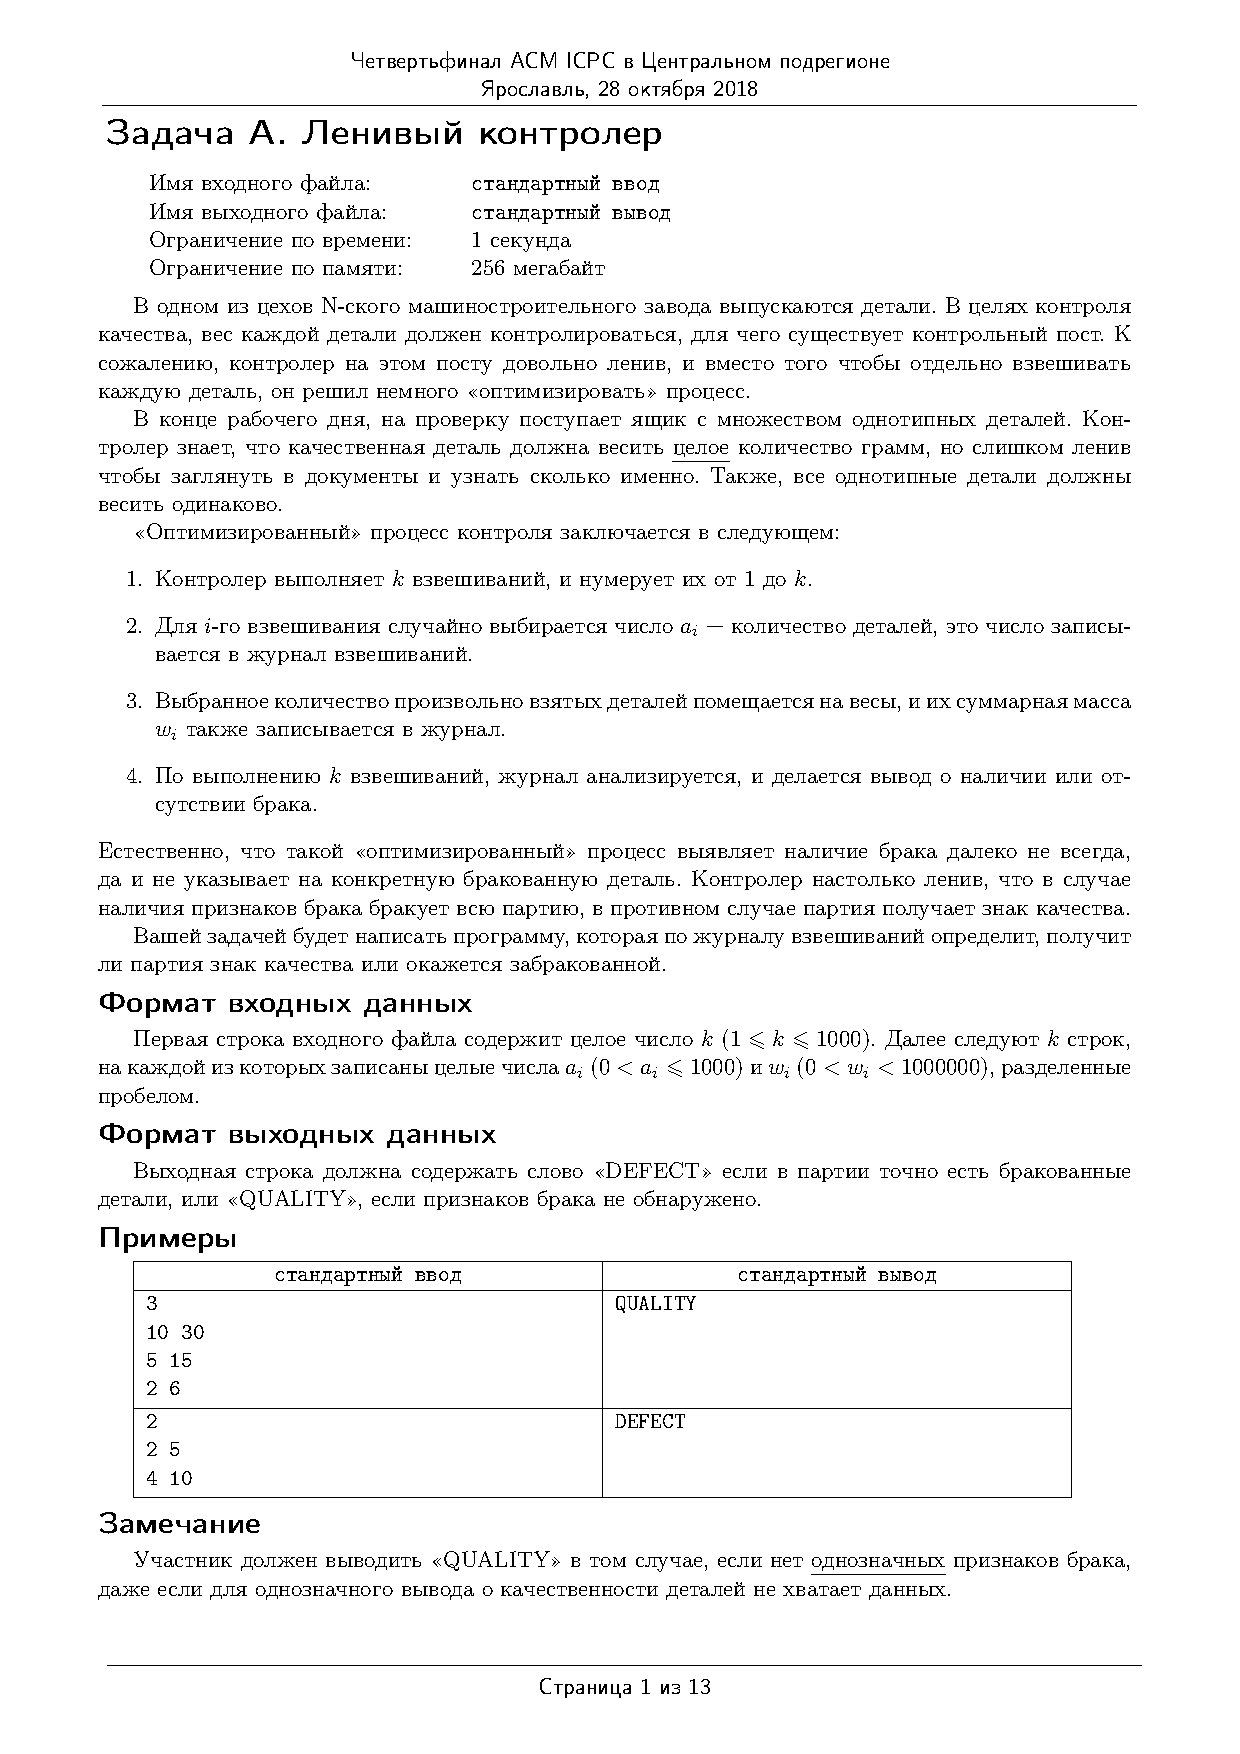
\includepdf[pages=1, scale=0.75, pagecommand=\section*{МАИ на CodeForces 20.03.22}]{statements/statements.pdf}
\subsection*{Идея}
Для данной задачи мы создаём переменную-индикатор $check$. Также мы создаём переменную $d$ - масса каждой детали предыдущего взвешивания отдельно. Далее мы последовательно считываем данные $a$ (число деталей), $w$ (их общая масса) в цикле. Если масса детали текущего взвешивания не равна целому числу, а также не соответсвует $d$, переменная $check$ становится $false$. Если переменная $check$ осталась $true$ после завершения цикла -  печатаем 'QUALITY', в противном случае - 'DEFECT'.
\subsection*{Исходный код}
\lstinputlisting{src/TaskA.cpp}
\subsection*{Фрагмент турнирной таблицы контеста}
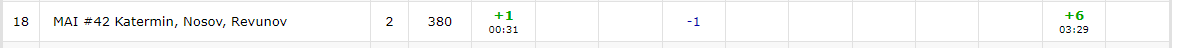
\includegraphics[scale=0.5]{standings/2003.png}\newline\noindent
\pagebreak

\section*{МАИ на CodeForces 27.03.22}
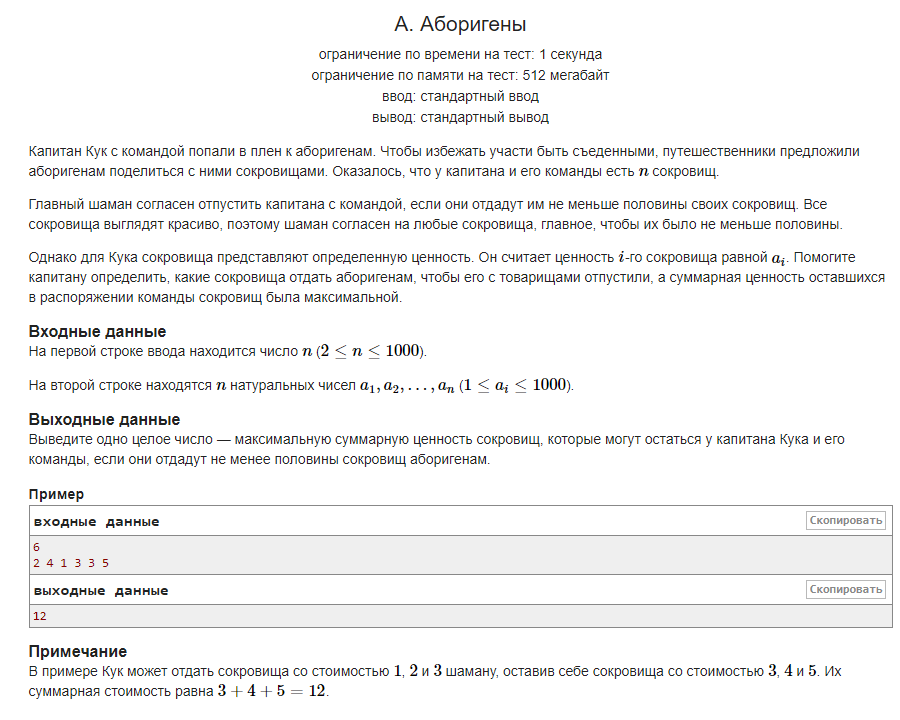
\includegraphics[scale=0.7]{statements/2703_A.png}\newline\noindent
\subsection*{Идея}
По заданию, отдать следует наименее ценные сокровища. Потому отсортируем их с помощью сортировки подсчётом по возрастанию и выведем первую половину. Чтобы не возникало с вопросом насчёт нечётного количества сокровищ, мы воспользуемся ухищрением, которая позволяет выполнить деление с округлением к большему - $i = (n-1)/2+1$, где "/" означает целочисленное деление. Под конец мы выводим сумму остального.
\subsection*{Исходный код}
\lstinputlisting{src/TaskA_2703.cpp}
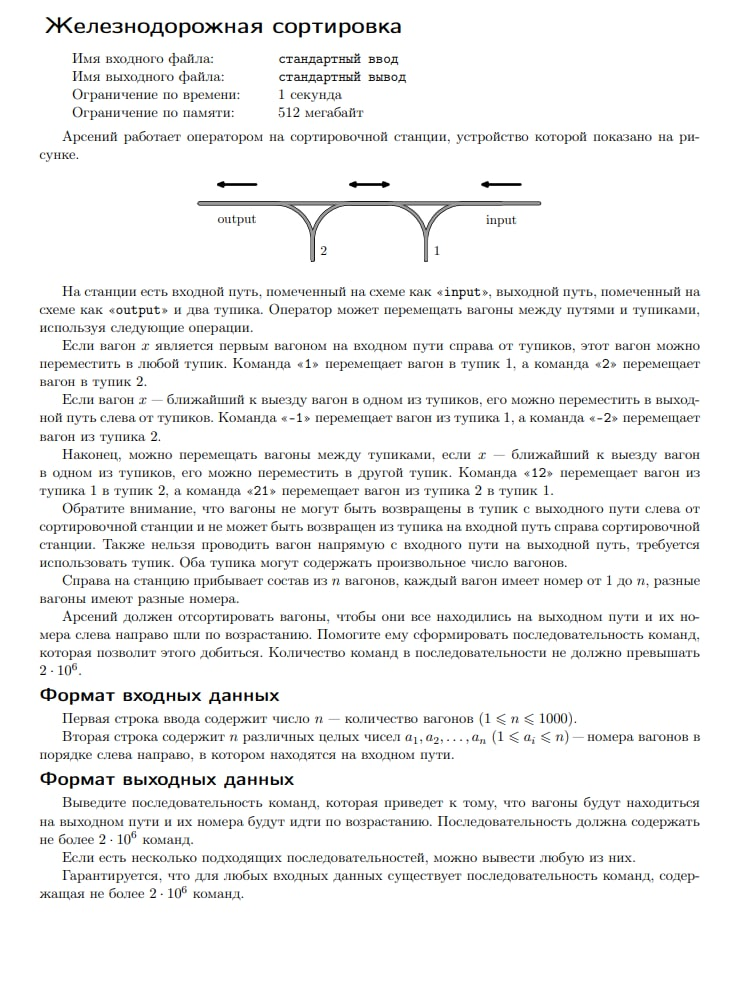
\includegraphics[scale=0.7]{statements/2703_K.jpg}\newline\noindent
\subsection*{Идея}
Берём два стека и очередь с исходными числами. Создаём массив, который показывает, где находится каждое число: в первом стеке, входной очереди или во втором стеке. Затем в цикле от 1 до $n$ смотрим, где находится $i$. Если в стеке - перекидываем все до нее во второй стек. И вытаскиваем само число на выход. Аналогично, если i находится во входной очереди: загружаем все во второй стек, пока не доберёмся до нужного нам значения.
\subsection*{Исходный код}
\lstinputlisting{src/TaskK_2703.cpp}
\subsection*{Фрагмент турнирной таблицы контеста}
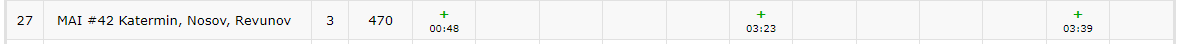
\includegraphics[scale=0.5]{standings/2703.png}\newline\noindent
\pagebreak

\includepdf[pages=3, scale=0.75, pagecommand=\section*{МАИ на CodeForces 03.04.22}]{statements/statements (03.04).pdf}
\subsection*{Идея}
Задача довольно простая. С помощью функции $permutations()$ модуля $itertools$ в Python мы проходим через все комбинации чисел (при этом изменяя их порядок) и сравниваем сумму первых двух чисел с третьим. Если мы находим такую комбинацию, то цикл останавливается с помощью команды $break$. В противном случае мы выводим "-1 -1 -1"
\subsection*{Исходный код}
\lstinputlisting[language=Python]{src/TaskC.py}
\subsection*{Фрагмент турнирной таблицы контеста}
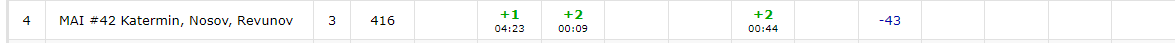
\includegraphics[scale=0.5]{standings/0304.png}\newline\noindent
\pagebreak

\includepdf[pages=13, scale=0.75, pagecommand=\section*{МАИ на CodeForces 10.04.22}]{statements/maratona_en.pdf}
\subsection*{Идея}
Для данной задачи мы создаём переменную-индикатор $check$. Также мы заводим два достаточно больших двухмерных вектора $v1$ и $v2$. В первый, по индексу цвета, мы записываем номер блока в под-вектор. Во второй, так же по индексу цвета, мы записываем индекс цикла в под-вектор. Оба действия мы выполняем в цикле $n$ (количество блоков) раз. Далее мы проходимся по векторам в цикле $k$ (количество цветов) раз. Сначала сортируем по возрастанию все непустые под-векторы первого вектора в порядке возрастания. Далее мы проходимся по каждому под-вектору обоих векторов и попарно их сравниваем. Если элементы не одинаковы, переменная $check$ становится $false$, и цикл останавливается. Если переменная $check$ осталась $true$ после завершения циклов -  печатаем 'Y', в противном случае - 'N'.

Сложность решения зависит от выбора функции сортировки, std::sort работает в среднем за $n \cdot log(n)$.
\subsection*{Исходный код}
\lstinputlisting{src/TaskH.cpp}
\includepdf[pages=18, scale=0.75]{statements/maratona_en.pdf}
\subsection*{Идея}
Для данной задачи мы создаём переменную-индикатор $check$, но на этот раз мы её задаём значение $false$. Также мы задаём переменную $sleep$ - номер минуты, начиная с которой мы начали спать. Далее мы в цикле читаем время выдачи еды ($x$), сравниваем разницу $x$ и $sleep$ и переменную $t$ (количество минут, которое нам необходимо поспать, чтобы выспаться) и если первое больше второго хотя бы один раз, переменная $check$ становится $true$. После цикла мы сравниваем разницу $d$ (длительность полёта) и $sleep$ и переменную $t$ с аналогичными условиями - проверяем, можно ли выспаться после последней выдачи еды. Если переменная $check$ стала $true$ после завершения циклов -  печатаем 'Y', в противном случае - 'N'.
\subsection*{Исходный код}
\lstinputlisting{src/TaskK.cpp}
\subsection*{Фрагмент турнирной таблицы контеста}
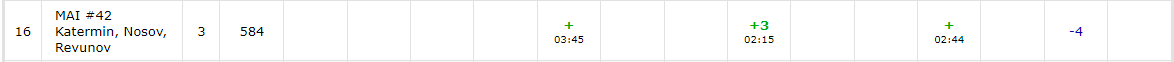
\includegraphics[scale=0.5]{standings/1004.png}\newline\noindent
\pagebreak

\section*{МАИ на CodeForces 17.04.22}
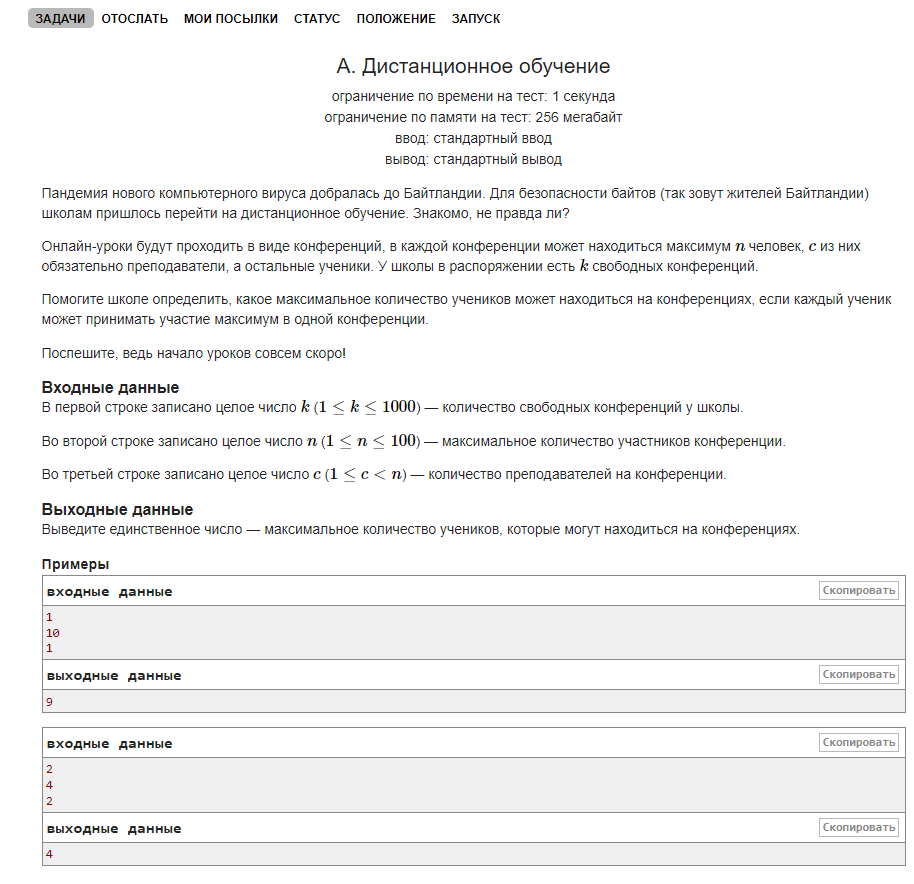
\includegraphics[scale=0.7]{statements/1704_A.png}\newline\noindent
\subsection*{Идея}
Задача проще пареной репы. Из количество участников мы вычитаем количество преподавателей, а полученный результат мы умножаем на количество конференций.
\subsection*{Исходный код}
\lstinputlisting{src/TaskA_1704.cpp}
\subsection*{Фрагмент турнирной таблицы контеста}
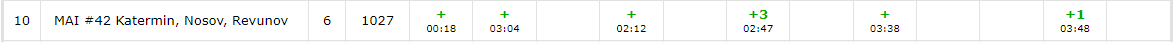
\includegraphics[scale=0.5]{standings/1704.png}\newline\noindent
\pagebreak

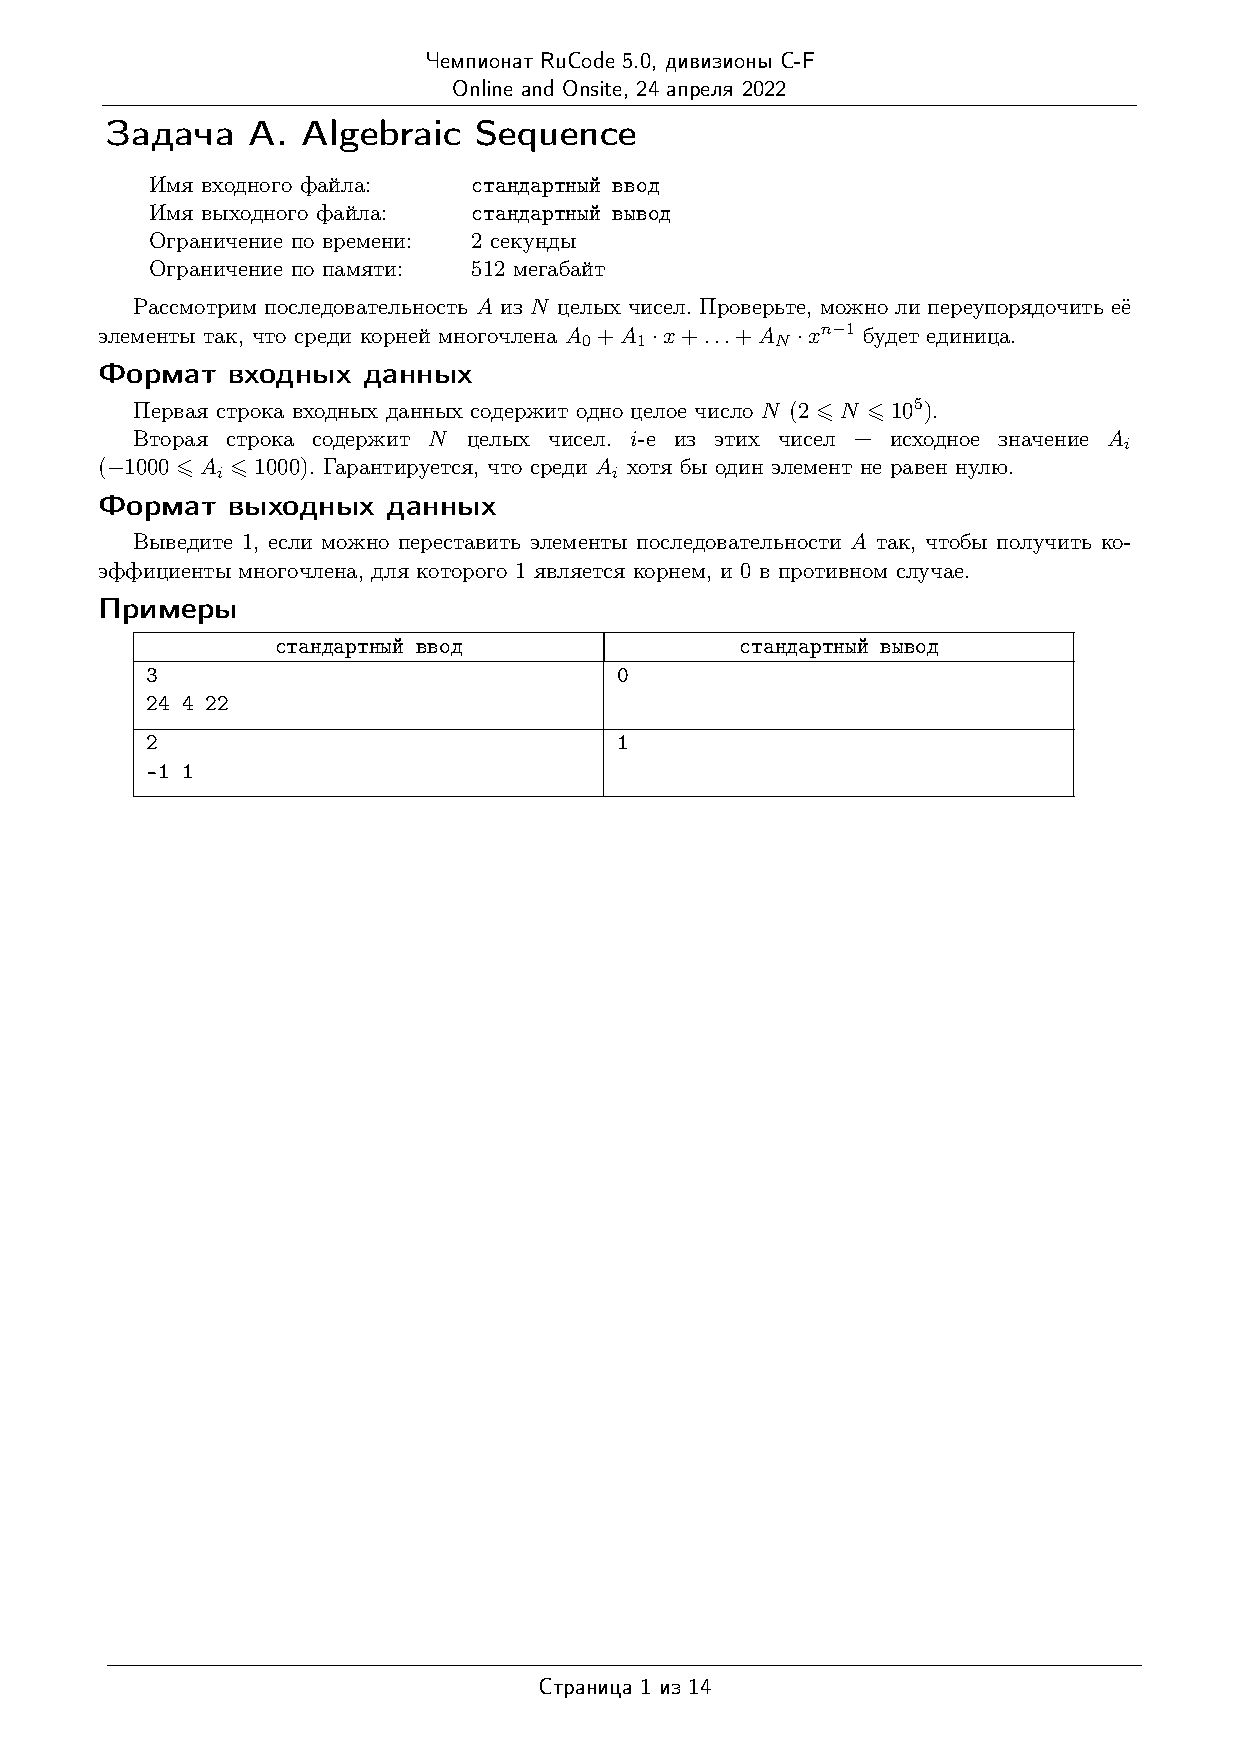
\includepdf[pages=1, scale=0.75, pagecommand=\section*{RuCode 5.0 Championship 24.04.2022}]{statements/cdef-ru.pdf}
\subsection*{Идея}
Было обнаружено, что для выполнения условия достаточно, что сумма всех элементов многочлена равна нулю.
\subsection*{Исходный код}
\lstinputlisting[language=Python]{src/TaskA_RC.py}
\subsection*{Фрагмент турнирной таблицы контеста}
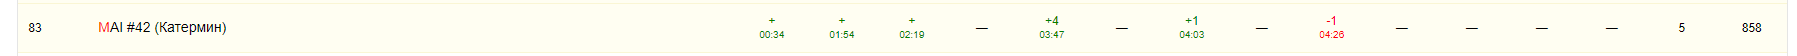
\includegraphics[scale=0.3]{standings/2404.png}\newline\noindent
\pagebreak

\includepdf[pages=6, scale=0.75, pagecommand=\section*{Grand Prix of BSUIR 01.05.2022}]{statements/1651364861935-contest-27097-en.pdf}
\subsection*{Идея}
Поскольку нам нужно отследить начало надписи, нужно отделить первую строку от остальных. Сначала мы проверяем, есть ли в строке 4 символа решётки, идущих подряд - у нас остаются первая, четвёртая и последняя строки. Затем мы проверяем, являются ли 20-й и 21-й символы (горизонтальные чёрточки у буквы I) символом решётки - теперь у нас остаются первая и последняя строки. Напоследок мы проверяем, являются ли 23-й и 24-й символы (где у буквы R есть сильные различия вверху и внизу) символом решётки. Если всё является верным, то мы нашли начало первой строки. Записываем его координаты в переменные $x$ и $y$ и выводим их.
\subsection*{Исходный код}
\lstinputlisting{src/TaskA0105.cpp}
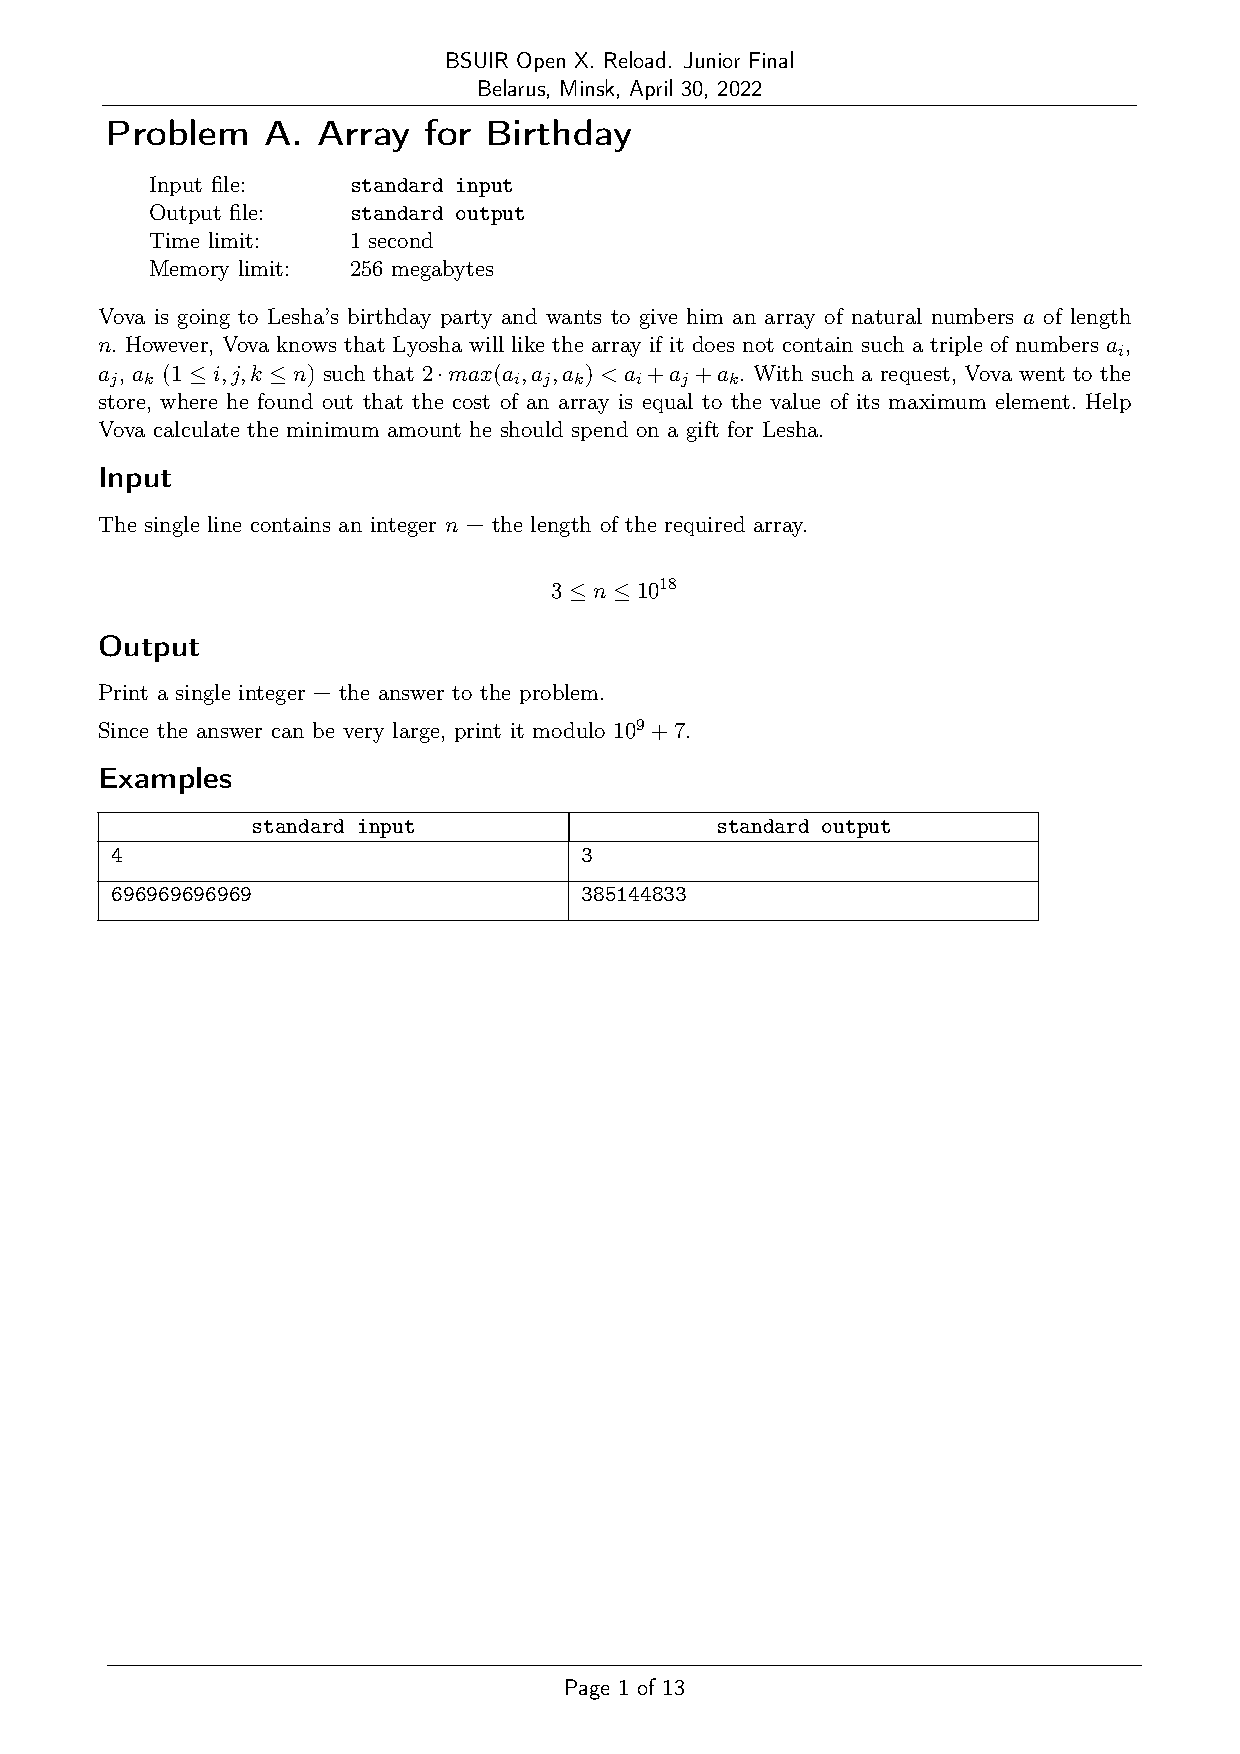
\includepdf[pages=1, scale=0.75]{statements/1651364861935-contest-27097-en.pdf}
\subsection*{Идея}
В этой задаче мы вычисляем Числа фибоначчи по модулю 1e9+7. В качестве способа подсчета мы используем бинарное возведение в степень n (матричным способом - представляет собой умножение заданной матрицы саму на себя n-ое количество раз, где n – степень, в которую необходимо возвести исходную матрицу. ) матрицы [0 1] [1 1] (по заданному модулю)
\subsection*{Исходный код}
\lstinputlisting{src/TaskA_0105.cpp}
\includepdf[pages=4, scale=0.75]{statements/1651364861935-contest-27097-en.pdf}
\subsection*{Идея}
Решение этой задачи сильно основывается на методе подсчета конечных нулей факториала числа в любой системе счисления. Алгоритм следующий:
\begin{center}  
  \item Разложить число $k$ системы счисления на простые множители;
  \item Разделить число $n$ на каждый уникальной простой множитель $s$, домножая $s$ сам на себя до тех пор, пока $n \over s$ будет больше единицы, при этом округляя каждый результат до меньшего целого;
  \item Если при разложении числа системы счисления мы получили несколько одинаковых простых множителей $s$, то результат выше мы должны разделить на количество одинаковых $kk$;
  \item Из всех делений $n$ на каждый уникальный множитель $kk$ выбрать наименьшее частное, которое и будет нашим ответом.
\end{center} 
\subsection*{Исходный код}
\lstinputlisting{src/TaskD.cpp}
\subsection*{Фрагмент турнирной таблицы контеста}
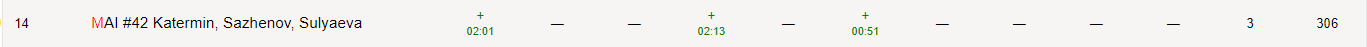
\includegraphics[scale=0.4]{standings/0105.png}\newline\noindent

\subsection*{Выводы}
Прошла обучение в олимпиадном программировании. Изучила основы плюсов и дп, теорию чисел, арифметику в кольце, комбинаторику, функции Эйлера, префиксные суммы, сортировка событий, метод двух указателей, научилась использовать библиотеки, приняла участие в опенкапах. Написала отчёт на LaTeX.
\pagebreak
